As mentioned in the abstract, the dichotomy between tight and overtwisted is a fundamental concept in contact geometry.
First insights about these attributes were gained when, early in the development of the field, 
Eliashberg discovered the ``overtwisted disk".
If a three-dimensional contact manifold admits an embedding of such a special disk, it is called overtwisted.
As mentioned in the abstract, such contact structures satisfy an $h$-principle.
An $h$-principle holds whenever a class of geometric structures is classified, 
up to homotopy, by its underlying topological structures (see \cref{sec:h_principle}).
In this case, the more general set are almost contact structures, where an almost contact structure
is simply the underlying topological structure of a contact structure.
Any such almost contact structure is homotopic to an overtwisted contact structure.
This is why overtwisted contact structures are comparably uninteresting: They exist
in abundance and can be classified by purely topological methods.

Contact structures that aren't overtwisted are called \textit{tight}.
Tight contact structures, however, are far more difficult to classify or even find than overtwisted ones.
Understanding tightness has therefore been a big motivating question in contact geometry.

The first systematic step in the direction of understanding tightness was the seminal work
by Eliashberg--Gromov \cite{Gromov85, Eliashberg91}. Using holomorphic curves, they proved that any type of fillability implies tightness.
Before moving on to the explanation of fillability, it is worth saying a few words on holomorphic curves.
Gromov's idea to use that technique for the proof was really visionary. 
Until today, all approaches for proving tightness are based on holomorphic curves.
The rough idea of Gromov--Eliashberg was to assume that there is a holomorphic disk, 
and then find a contradiction by constructing a suitable moduli space of holomorphic disks.
Nowadays, tools like contact homology (or similar homology theories) are all based on holomorphic curves, too.

Fillability is another important aspect of contact geometry, based on its relation to symplectic geometry.
While contact manifolds are always odd-dimensional, symplectic geometry is the corresponding concept in even dimensions.
Manifolds that are equipped with a closed nondegenerate 2-form are called symplectic. They are related
to contact manifolds in many ways.
For example, a hypersurface in a contact manifold with a transversal contact vector field
induces a convex splitting of this hypersurface: There is the so-called dividing set (a contact submanifold)
which divides the hypersurface into Liouville domains, i.e. exact symplectic manifolds (cf. \cref{sec:convex_decomposition}).

The main connection between symplectic and contact manifolds, however, is the concept of fillability:
A contact manifold is (strongly) fillable if it is the smooth boundary of a symplectic manifold and
near the boundary, there is a Liouville vector field pointing outwards at the boundary.
For example, the standard contact structure on the sphere $(S^3, \xi)$ is fillable
by the standard symplectic structure on the ball $(B^4, \omega)$.

Now, as the word ``strongly" already suggests, there are several variants of fillability:
A contact manifold can be (Wein-)Stein fillable, Liouville fillable, (strongly) fillable or weakly fillable.
From left to right, there are less and less conditions to be satisfied, i.e. there is a sequence
of implications from the left to the right. 
Eliashberg--Gromovs result adds tightness to the right end of these implications.

In other words, there is a chain of inclusions from 
Weinstein- and Liouville- over strongly and weakly fillable to tight contact manifolds.
In three dimensions, these inclusions were all proven to be strict, see \cref{fig:fillability}.
\begin{figure}
    \begin{align*}
        \{\text{Weinstein fillable}\} \stackrel{\text{\cite{Bowden12}, \cite{BCS14}}}{\subsetneq} 
        \{\text{Liouville fillable}\} \stackrel{\text{\cite{Ghiggini05}, \cite{Zhou21}}}{\subsetneq}\\
        \{\text{Strongly  fillable}\} \stackrel{\text{\cite{Eliashberg96}, \cite{BGM22}}}{\subsetneq}
        \{\text{Weakly    fillable}\} \stackrel{\text{\cite{EH02}, \cite{MNW13}}}{\subsetneq}
        \{\text{Tight}\}
    \end{align*}
    \caption{Hierarchy of fillability in three dimensions (first citation) and in higher dimensions (second citation)}
    \label{fig:fillability}
\end{figure}

Basically all of the concepts explained before have been generalized to higher dimensions.
One example where this was not straightforward is the generalization of overtwistedness: 
After a long process, multiple potential definitions were shown to be equivalent in arbitrary dimensions \cite{BEM15,CMP19,Huang17}.

Another example is that there is a similar hierarchy of fillabilities in higher dimensions. 
Most definitions generalize to higher dimensions in a straightforward way. Tightness can just be defined as \textit{not overtwisted}.
It turns out that the same chain of inclusions is true in higher dimensions, too.
Proving the strictness of these inclusions took another few years, but now all inclusions are known to be strict also in higher dimensions, 
see \cref{fig:fillability}.

Often, however, these proofs of strictness simply construct very specific counterexamples with a very specific underlying smooth manifold.
This leads to the question whether the strictness of these inclusions is due to specific geometric properties of the counterexamples.
Bowden--Gironella--Moreno--Zhou \cite{BGMZ22} provide a negative answer to this question by showing that tight but
non-fillable contact structures exist in every almost contact class that admits a tight structure (in $\dim = 5$, there is an additional assumption, namely $c_1\neq 0$).
This proves that there really is a inherently contact geometric difference between tightness and fillability
that can't be attributed to specific properties of the underlying smooth topology.

The proof starts with first establishing a more specific theorem: There are homotopically standard, tight, but non-fillable contact structures on the sphere.
Then, by so called ``contact connected sum" (a connected sum operation that respects the contact structure),
the general result follows.

Also, they prove that any sphere in $\dim \geq 7$ admits homotopically standard Liouville- but not Weinstein-fillable contact structures
and, analogously, deduce a more general statement from this via contact connected sum.
As weak and strong fillability are equivalent on the sphere, there are two remaining questions along this line of research:
\begin{itemize}
    \item Is there a Liouville- but not Weinstein-fillable contact structure on $S^5$?
    \item Does a higherdimensional sphere admit strongly, but not Liouville-fillable contact structures?
\end{itemize}

This thesis focuses on the first theorem of \cite{BGMZ22}: $S^{2n+1}$ admits a homotopically standard, tight, but non-fillable contact structure
for any $n \geq 2$. In fact, as the case for $n = 2$ is similar, but technically more difficult, it is omitted.

The chapters of this thesis correspond to the three main steps of the proof. First, one constructs a homotopically standard contact structure on $S^{2n+1}$.
This contact structure is then, secondly, shown to be tight.
Thirdly, non-fillability is deduced.

The starting point of \cref{chap:construction} is the famous Giroux-correspondence.
Giroux disvovered that contact structures are closely related with open book decomposition.
An open book decomposition really is a very intuitive concept: In a manifold $M^n$, find a codimension two submanifold $B^{n-2}$
s.t. there is a fibration $p\colon M\setminus B \to S^1$. $B$ is then called ``binding" and the fibers $p^{-1}(\theta)$ are the pages of the open book 
(see \cref{fig:open_book}).

\begin{figure}
    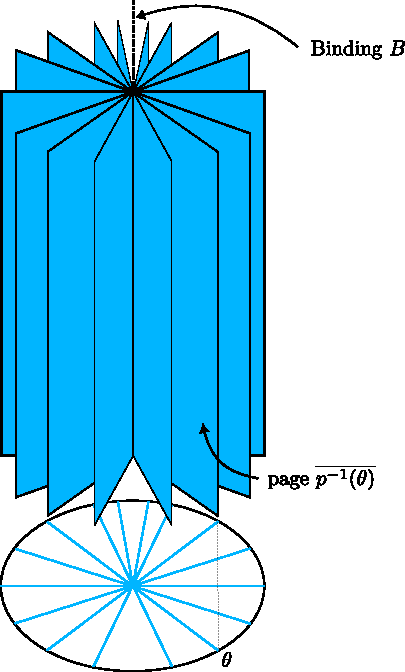
\includegraphics{../images/open_book.pdf}
    \caption{Open Book Decomposition}
    \label{fig:open_book}
\end{figure}

The Giroux correspondence states that in 3 dimensions, there is a bijection (modulo technical details) between contact structures
and open book decompositions.
In higher dimensions, similar statements hold, in particular any open book decomposition leads to a corresponding supported
contact structure via the Thurston-Winkelnkemper-construction.
This is used in the proof in order to construct a contact structure that is different from the standard contact structure on $S^{2n+1}$.

Constructing a tight contact structure is not so easy: The standard way would be to take the boundary of some symplectic manifold,
but then it is of course fillable, so this approach can't be used here.
Even though there are many procedures that make a contact structure overtwisted (e.g. adding a Lutz twist), tightening procedures are very rare.
Only the Bourgeois construction was known to often yield tight contact structures. 
A recent preprint by Avdek and Zhou now proves that, in fact, Bourgeois manifolds are always tight \cite{AZ24}.
Therefore, the next step in the proof is to apply the Bourgeois construction, resulting in a Bourgeois manifold $S^{2n-1} \times T^2$.
Clearly, this has the wrong topology, so the final step in the construction is to kill the $T^2$-factor with
subcricital contact surgeries, establishing a homotopically standard contact structure on the sphere $(S^{2n+1},\xi_\text{new})$.

In \cref{chap:tightness}, one uses Reeb dynamics and holomorphic curves hidden in the framework of contact homology to prove that $\xi_\text{new}$
is really tight.

Finally, \cref{chap:nonfillable} finds a contradiction if the manifold was fillable. So first, assume it is fillable.
The largest part then is devoted to proving that fillability implies a certain property for specific homology classes
(the homological obstruction theorem).
As the theorem is easier to prove for $S^{2n-1} \times T^2$ instead of the surgered manifold $S^{2n+1}$,
this thesis covers only the proof for the homological obstruction theorem for $S^{2n-1} \times T^2$ according to \cite{BGM22}. 
The proof in the general case is similar.
Then, in the final section, a homology class as described in the homological obstruction theorem is constructed.
However, it doesn't satisfy the required property, thus establishing the desired contradiction.